% Figure 4.5 (Session 4): the AKLT picture of the spin-1 chain and its edge moments.
% The image is rendered by figures/blender/s4_5_aklt.py; the coordinates of the labels come from
% figures/blender/out/aklt_anchors.tex. Compile with:
%   pdflatex aklt.tex ; result moves to ../mps_spin_chains/aklt.pdf
\documentclass[11pt,tikz,border=0pt]{standalone}
\usepackage{amsmath,amssymb,graphicx}
\usepackage{xcolor}
\definecolor{coursedark}{HTML}{1B2A4A}
\definecolor{costamber}{HTML}{B8620A}
\newlength{\figw}\setlength{\figw}{16.19cm}   % the text width of the notes (letter, 2.7 cm margins), so labels print at size

\begin{document}
\begin{tikzpicture}[lbl/.style={font=\small, text=coursedark}]
  \node[anchor=south west, inner sep=0pt] at (0,0)
    {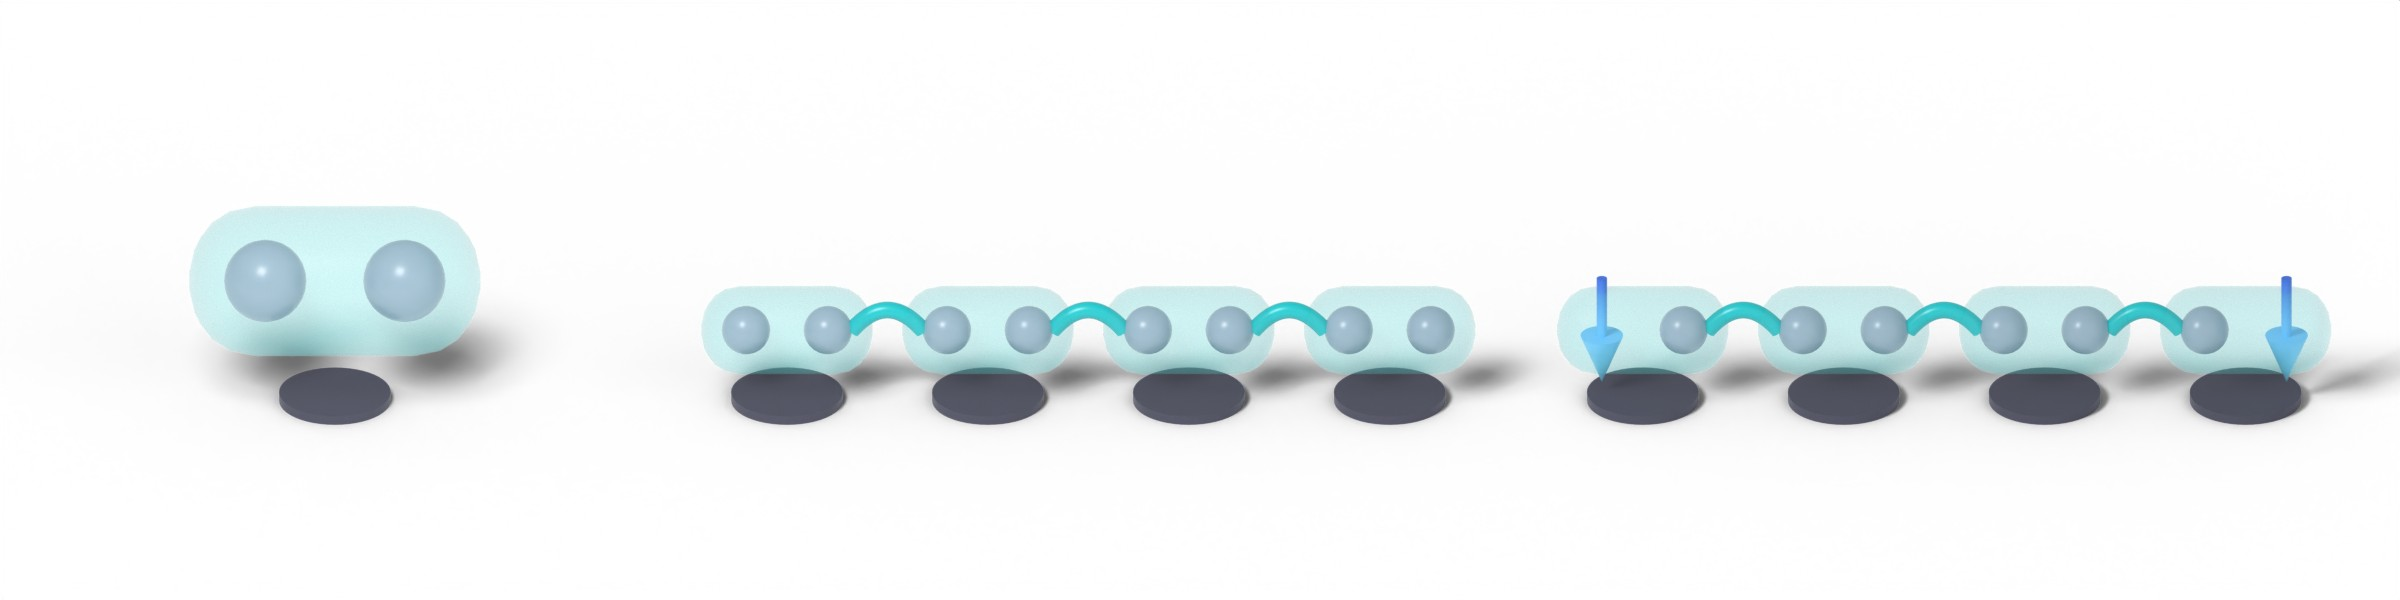
\includegraphics[width=\figw]{../blender/out/aklt.jpg}};
  %% written by figlib.py; x and y in units of the image width
\coordinate (a) at (0.0465\figw,0.2051\figw);
\coordinate (aS1) at (0.1395\figw,0.1761\figw);
\coordinate (ahalf) at (0.1395\figw,0.0628\figw);
\coordinate (b) at (0.2698\figw,0.2051\figw);
\coordinate (bsing) at (0.4535\figw,0.1264\figw);
\coordinate (blbl) at (0.4535\figw,0.0628\figw);
\coordinate (c) at (0.6264\figw,0.2051\figw);
\coordinate (cleft) at (0.6674\figw,0.0679\figw);
\coordinate (cright) at (0.9527\figw,0.0679\figw);

  \node[lbl, font=\normalsize, anchor=west] at (a) {(a)};
  \node[lbl, font=\normalsize, anchor=west] at (b) {(b)};
  \node[lbl, font=\normalsize, anchor=west] at (c) {(c)};
  \node[lbl, anchor=south] at (aS1) {$S=1$};
  \node[lbl, anchor=north] at (ahalf) {two spin-$\tfrac12$};
  \node[lbl, anchor=south] at (bsing) {singlet};
  \node[lbl, anchor=north] at (blbl) {valence bonds};
  \node[lbl, anchor=north] at (cleft) {\normalsize $-\frac{1}{2}$};
  \node[lbl, anchor=north] at (cright) {\normalsize $-\frac{1}{2}$};
\end{tikzpicture}
\end{document}
